\documentclass[12pt,a4paper]{article}
% !TEX program = xelatex
\usepackage[utf8]{inputenc}
\usepackage[T1]{fontenc}
\usepackage[finnish]{babel}
\usepackage[utf8]{inputenc}
\usepackage{graphicx}
\usepackage{titling}
\usepackage{titlesec}
\usepackage{booktabs}
\usepackage{fancyhdr}
\usepackage{lipsum}
\usepackage{comment, mdframed}
\usepackage{enumitem}
\usepackage{xcolor}
\usepackage{longtable}
%\usepackage{cite}
\usepackage{pgfgantt}
\usepackage{amsmath, amssymb}
\usepackage{tikz}
\usepackage[margin=1in]{geometry}
\usepackage[backend=biber, style=numeric]{biblatex}
%\usepackage{hyperref}
\usepackage{bookmark}
\usepackage{enumitem}
\usepackage{amsmath}
\usepackage{listings}
\lstset{language=Python, basicstyle=\ttfamily\small, breaklines=true,columns=fullflexible}
\lstset{escapeinside={(*@}{@*)}}
\usepackage{fontspec}
\setmainfont{Arial}
\newfontfamily\stylishfont{Noteworthy}
%\newfontfamily\stylishfont{Zapfino}
%\addbibresource{references.bib}
\usetikzlibrary{calc}
\usepackage{xcolor}

\lstdefinestyle{pidstyle}{
    basicstyle=\ttfamily\footnotesize,
    breaklines=true,
    escapechar=\#, % Define escape character for inline LaTeX commands
    linewidth=\textwidth,
    basicstyle=\ttfamily\scriptsize
}

\renewcommand{\maketitle}{%
  \begin{leftmark}
    \vspace*{\baselineskip} % Add a bit of vertical space

%    \includegraphics[width=4cm]{example-image-a} % Add an image before the title. you will need to replace the image path with your own

%    \vspace{0.5cm} % Add vertical space before title

    \textbf{\fontsize{18}{36}\selectfont \thetitle} % Font Size and Bold Title

     \vspace{0.05cm} % Add vertical space before subtitle
%    \textit{\Large \theauthor}  % Subtitle / Author
    \vspace{\baselineskip} % Add vertical space after subtitle
     \rule{\textwidth}{0.4pt} % Add a horizontal line

   \end{leftmark}
%    \thispagestyle{empty} % Prevent header/footer on the title page
}


% Section Formatting
\titleformat{\section}
  {\normalfont\fontsize{18}{22}\bfseries} % Font and style
  {\thesection}         % Section number
  {1em}                   % Horizontal space after section number
  {}                     % Code before the section name
  []                     % Code after the section name

\titleformat{\subsection}
  {\normalfont\fontsize{14}{18}\bfseries} % Font and style
  {\thesubsection}         % Subsection number
  {1em}                   % Horizontal space after subsection number
  {}                     % Code before the subsection name
  []                     % Code after the subsection name

\setlength{\parindent}{0pt}

\title{Computing platforms (Spring 2025)\newline
week 6}
\author{Juha-Pekka Heikkilä}



\pagestyle{fancy}
\fancyhf{}

\renewcommand{\headrulewidth}{0pt}

\newcommand{\footerline}{\makebox[\textwidth]{\hrulefill}}

\newcommand{\footercontent}{%
    \begin{tabular}{@{}l@{}}
        \footerline \\
        \leftmark \hfill \rlap{\thepage}
    \end{tabular}
}

\fancyfoot[C]{\footercontent}


\newcommand{\exercise}[1]{
    \section*{Tehtävä #1}
    \markboth{Tehtävä #1}{}
}

\addtolength{\hoffset}{-1.75cm}
\addtolength{\textwidth}{3.5cm}
%\addtolength{\voffset}{-3cm}
%\addtolength{\textheight}{6cm}
%\setlength{\parindent}{0pt}



% (a), (b), (c)
\newlist{kohta}{enumerate}{1}
\setlist[kohta,1]{
  label=\textbf{\makebox[1cm][l]{\Huge\text{(\stylishfont\alph*)}}},
  leftmargin=!,
  labelindent=0pt
}

% (1), (2), (3)
\newlist{alakohta}{enumerate}{1}
\setlist[alakohta,1]{
  label=\textbf{\makebox[1cm][l]{\Large\text{(\arabic*)}}},
  leftmargin=!,
  labelindent=0pt
}

% termi: selitys
\newlist{kuvaus}{description}{1}
\setlist[kuvaus]{%
  font=\bfseries\stylishfont,
  labelsep=0.5cm,
  leftmargin=2.5cm,
  style=nextline
}

\newcommand{\korostus}[2][yellow]{\colorbox{#1}{\strut #2}}
%\korostus{Yksi kirjoittaja on jo sisällä}
%\korostus[red]{Lukijan täytyy odottaa jos kirjoittajia on paikalla}
%\korostus[orange]{Tämä osa ei ole suoritettavissa}


\newcommand{\evalslantti}[4][-12]{%
%  \left. #2 \,\right|% ei indeksejä tähän
  \mkern-10mu\raisebox{0pt}[0pt][0pt]{\rotatebox{#1}{$\Big|$}}% vinoviiva päälle
  \mkern3mu{}_{\!#3}^{\!#4}% arvot viivan oikealle puolelle
}


\newcommand{\evalraise}{1.2ex}
\newcommand{\evallow}{1.2ex}

% vino eval-viiva, arvot oikealla (oletus: -12)
% \evalslant[asteet]{lauseke}{ala}{yla}
\newcommand{\evalslant}[4][-12]{%
  \left. #2 \,\right.%
  \mkern-10mu\raisebox{0pt}[0pt][0pt]{\rotatebox{#1}{$\Big|$}}%
  \mkern2mu{}^{\raisebox{\evalraise}{$\scriptstyle #4$}}_{\raisebox{-\evallow}{$\scriptstyle #3$}}%
}



% vino eval-viiva ENNEN lauseketta
% \evalslantpre[asteet]{lauseke}{ala}{yla}
\newcommand{\evalslantpre}[4][-12]{%
  % viiva ja rajat
  \raisebox{0pt}[0pt][0pt]{\rotatebox{#1}{$\Big|$}}%
  \mkern2mu{}^{\raisebox{\evalraise}{$\scriptstyle #4$}}_{\raisebox{-\evallow}{$\scriptstyle #3$}}%
  % itse lauseke
  \mkern4mu\left. #2 \right.%
}


\DeclareMathOperator{\Var}{Var}
\DeclareMathOperator{\Cov}{Cov}
\DeclareMathOperator{\Corr}{Corr}
\usepackage{tikz}
\usetikzlibrary{automata, positioning, arrows.meta}
\usepackage{amssymb,amsmath,graphicx,color}
\usepackage{forest}

\newcommand{\set}[1]{\left\{\,#1\,\right\}}
\newcommand{\abs}[1]{\lvert#1\rvert}

\newcommand{\N}{\mathbb{N}}
\newcommand{\Pot}{{\cal P}}

\newcommand{\rma}{\mathrm{a}}
\newcommand{\rmb}{\mathrm{b}}
\newcommand{\rmc}{\mathrm{c}}

\title{TKT20005 Laskennan mallit Viikko4}
\date{}

\begin{document}

\maketitle

\exercise{1 Säännöllisten lausekkeiden muodostaminen.}
Esitä säännöllinen lauseke seuraaville aakkoston
$\Sigma=\set{\rma,\rmb,\rmc}$ kielille:
\begin{kohta}
\item merkkijonot, joissa joka toinen merkki on b (joka toinen merkki tarkoittaa tässä merkkejä numero 2, 4, 6 jne., mikäli merkkijonossa on ainakin niin monta merkkiä)
\[
\big((\mathrm{a}\mid\mathrm{b}\mid\mathrm{c})\,\mathrm{b}\big)^{*}\,(\,\varepsilon\mid\mathrm{a}\mid\mathrm{b}\mid\mathrm{c}\,)
\] 
\item merkkijonot, joissa on pariton määrä c-merkkejä
\[
(\mathrm{a}\mid\mathrm{b})^{*}\ \mathrm{c}\ \big((\mathrm{a}\mid\mathrm{b})^{*}\ \mathrm{c}\ (\mathrm{a}\mid\mathrm{b})^{*}\ \mathrm{c}\big)^{*}\ (\mathrm{a}\mid\mathrm{b})^{*}
\]
\item merkkijonot, joissa on korkeintaan yhtä merkkiä
\[
\varepsilon \ \mid\ \mathrm{a}\ \mid\ \mathrm{b}\ \mid\ \mathrm{c}
\]
\item merkkijonot, joissa on ainakin kahta eri merkkiä
\[
(\mathrm{a}\mid\mathrm{b}\mid\mathrm{c})^{*}\,(\ \mathrm{ab}\mid\mathrm{ba}\mid\mathrm{ac}\mid\mathrm{ca}\mid\mathrm{bc}\mid\mathrm{cb}\ )\,(\mathrm{a}\mid\mathrm{b}\mid\mathrm{c})^{*}
\]
\item merkkijonot, jotka sisältävät osamerkkijonon abc
\[
(\mathrm{a}\mid\mathrm{b}\mid\mathrm{c})^{*}\ \mathrm{abc}\ (\mathrm{a}\mid\mathrm{b}\mid\mathrm{c})^{*}
\]
\item merkkijonot, jotka eivät sisällä osamerkkijonoa abc.
\[
\Big( (\mathrm{b}\mid\mathrm{c})^{*}\,\big(\ \mathrm{a}(\mathrm{a}\mid\mathrm{c})\ \mid\ \mathrm{ab}(\mathrm{a}\mid\mathrm{b})\ \big) \Big)^{*}\,
(\mathrm{b}\mid\mathrm{c})^{*}\,(\varepsilon\mid \mathrm{a})
\]
\end{kohta}






\pagebreak
\exercise{2 Muunnos säännöllisestä lausekkeesta äärelliseksi automaatiksi.}
Kieli $L=(0\cup 01)^{*}\subseteq\{0,1\}^*$ koostuu sanoista, joissa jokainen $1$ on heti
edeltävän $0$:n perässä (ei aloiteta $1$:llä, ei kahta peräkkäistä $1$:tä).

\begin{kohta}
\item DFA

\begin{center}
  \includegraphics[width=.4\textwidth]{viikko4tehtävä2_1.jpg}
\end{center}
\begin{comment}
    
\begin{center}
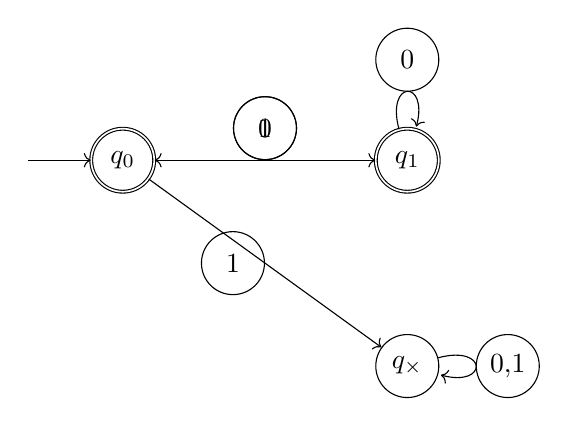
\begin{tikzpicture}[
  node distance=28mm,
  every node/.style={circle,draw,minimum size=8mm,inner sep=0pt}
]
\node (q0) [double] {$q_0$};                 % start, accept (ε)
\node (q1) [right=of q0, double] {$q_1$};     % just read 0 (still accept)
\node (qd) [below=18mm of q1] {$q_\times$};   % sink

\draw[->] (-1.2,0) -- (q0);

\draw[->] (q0) -- node[above] {0} (q1);
\draw[->] (q0) -- node[left]  {1} (qd);

\draw[->] (q1) edge[loop above] node {0} (q1);
\draw[->] (q1) -- node[above] {1} (q0);

\draw[->] (qd) edge[loop right] node {0,1} (qd);
\end{tikzpicture}
\end{center}
\end{comment}

\smallskip
Tää DFA hyväksyy $L$:n: $q_0$ ja $q_1$ ovat hyväksyviä (tyhjä sana ja
kaikki tähän asti validit päätökset), $1$ alussa tai $1$ ilman edeltävää $0$:aa
vie virheeseen

\item \emph{NFA lausekkeesta \((0\cup 01)^*\) luentomenetelmällä.}
(Käytetään $\varepsilon$-siirtymiä: tähti palaa alkuun, yhdiste haaroittaa.)

\begin{center}
  \includegraphics[width=.4\textwidth]{viikko4tehtävä2_2.jpg}
\end{center}


\pagebreak

\item DFA NFA:sta 
$\varepsilon$-sulut: $(s)=\{s,x,y\}$, muilla ei $\varepsilon$-siirtymiä.
Saavutettavat osajoukot ja siirtymät (hyväksyvä jos joukossa on $s$):

\[
\renewcommand{\arraystretch}{1.15}
\begin{array}{c|cc}
\text{DFA-tila} & 0 & 1\\\hline
\{s,x,y\}^\star     & \{s,x,y,z\}^\star & \varnothing \\
\{s,x,y,z\}^\star   & \{s,x,y,z\}^\star & \{s,x,y\}^\star \\
\varnothing         & \varnothing       & \varnothing
\end{array}
\]

\noindent Tästä saadaan DFA (isomorfinen edellä olevaan pieneen DFA:han):

\begin{center}
  \includegraphics[width=.4\textwidth]{viikko4tehtävä2_3.jpg}
\end{center}



\item Vertailu. DFA on sama kuin tehty pieni DFA:
\[
\{s,x,y\}\leftrightarrow q_0,\qquad
\{s,x,y,z\}\leftrightarrow q_1,\qquad
\varnothing\leftrightarrow q_\times.
\]
Molemmissa on kaksi hyväksyvää tilaa ja virhe, siirtymät:
$0$: $q_0\!\to\!q_1$, $q_1\!\to\!q_1$; \quad
$1$: $q_0\!\to\!q_\times$, $q_1\!\to\!q_0$.
\end{kohta}






\pagebreak
\exercise{3 Yhteydettömän kieliopin muodostaminen.}
Esitä yhteydettömät kieliopit, jotka tuottavat seuraavat
aakkoston $\Sigma=\set{0,1}$ kielet:
\begin{kohta}
\item
parittoman mittaiset merkkijonot
\[
S \to 0 \mid 1 \mid 0S0 \mid 0S1 \mid 1S0 \mid 1S1
\]

\item merkkijonot, joissa on osamerkkijono 111
\[
S \to X\,111\,Y,\qquad
X \to 0X \mid 1X \mid \varepsilon,\qquad
Y \to 0Y \mid 1Y \mid \varepsilon
\]
\item
merkkijonot, joissa on ainakin kaksi merkkiä ja joiden
ensimmäinen ja viimeinen merkki ovat samat
\[
S \to 0T0 \mid 1T1,\qquad
T \to 0T \mid 1T \mid \varepsilon
\]

\item $\set{0^n1^m\mid\mbox{$m,n\in\N$ ja $m\geq n$}}$
\[
S \to 0S1 \mid T,\qquad
T \to 1T \mid \varepsilon
\]

\item $\set{0^n1^k0^m\mid\mbox{$m,n,k\in\N$ ja $k=n+m$}}$
\[
S \to 0S1 \mid U,\qquad
U \to 1U0 \mid \varepsilon
\]

\end{kohta}






\pagebreak
\exercise{4 Yhteydetön kielioppi, jäsennyspuu ja johto.}
  
Tarkastellaan yhteydetöntä kielioppia
\begin{eqnarray*}
S&\rightarrow& SAB\mid\varepsilon\\
A&\rightarrow& \mathrm{a}A\mid\mathrm{a}\\
B&\rightarrow& \mathrm{b}B\mid\varepsilon
\end{eqnarray*}
Esitä merkkijonolle $\mathrm{aa}$ kaksi erilaista
jäsennyspuuta ja kummallekin sitä vastaava johto.

\bigskip

\begin{alakohta}
\item versio 1 (yksi $A$ tuottaa kaksi a:ta):

\begin{forest}
for tree={align=center, parent anchor=south, child anchor=north, l sep=8pt, s sep=6pt}
[S
  [S [\(\varepsilon\)]]
  [A
    [\(\mathrm{a}\)]
    [A [\(\mathrm{a}\)]]
  ]
  [B [\(\varepsilon\)]]
]
\end{forest}

\[
\begin{aligned}
S &\Rightarrow S A B \Rightarrow \varepsilon A B
   \Rightarrow \mathrm{a}A\,B \Rightarrow \mathrm{a}\mathrm{a}\,B
   \Rightarrow \mathrm{a}\mathrm{a}\,\varepsilon \;=\; \mathrm{aa}
\end{aligned}
\]

\item versio 2 (kaksi $A$-lohkoa, kumpikin tuottaa yhden a:n)

\begin{forest}
for tree={align=center, parent anchor=south, child anchor=north, l sep=8pt, s sep=6pt}
[S
  [S
    [S [\(\varepsilon\)]]
    [A [\(\mathrm{a}\)]]
    [B [\(\varepsilon\)]]
  ]
  [A [\(\mathrm{a}\)]]
  [B [\(\varepsilon\)]]
]
\end{forest}

\[
\begin{aligned}
S &\Rightarrow S A B \Rightarrow S A B\, A B
   \Rightarrow \varepsilon A B\, A B
   \Rightarrow \mathrm{a} B\, A B \Rightarrow \mathrm{a}\varepsilon\, A B \\
  &\Rightarrow \mathrm{a} A B \Rightarrow \mathrm{a}\mathrm{a} B
   \Rightarrow \mathrm{a}\mathrm{a}\varepsilon \;=\; \mathrm{aa}
\end{aligned}
\]
\end{alakohta}



\end{document}